\chapter{First Iteration}
\label{ch:firstiteration}
The solution to the stated problem was approached in an iterative manner. This section describes the first iteration, which focuses on laying the groundwork for future work. Because of this, the model produced is rather abstract.

The iteration was split into 4 major steps:

\begin{enumerate}
\item Design and implement a UPPAAL Cora model simulating the FESTO system
\item Make UPPAAL Cora and Python 3.5 cooperate
\item Use Python to Generate valid model configurations that  produce specific products
\item Pick out the best configuration out of a pool of candidates
\end{enumerate}

In the following we go over each of these steps in further detail.

\section{Design and Implementation in UPPAAL Cora}
For our models we use UPPAAL, an integrated tool environment used for modeling, simulating and verifying real time systems. When a model has been constructed, the model checker may be used to query invariant and reachability properties of the model.  We choose UPPAAL, as we have previous experience with it as well as the theory of timed automatas. In addition, many of its developers are located in Aalborg University along with the project group. Thus there is easy access to technical advice.  

After a FESTO factory has been modelled, we may query it about its properties. The most interesting property is one of reachability. Is it possible to reach a state, where  x amount of products have been produced? If this is the case, UPPAAL may produce a shortest timed trace of actions needed to reach this state.  However, the fastest trace isn’t always the best. For instance, a very fast trace may have the factory use up a lot of power. Thus, we are not only interested in high throughput, but also a low cost. In order to involve costs, we do not use plain UPPAAL for our models, but instead an offshoot named UPPAAL Cora. 

This program is very similar to regular UPPAAL, but it also allows for a single global cost variable to be used alongside the familiar global clock. This variable may only be increased. This can happen either when an action is taken, or as a function of time, when waiting in a location. The model checker may explore the state space in a UPPAAL Cora model in a Best First manner. That is, it looks for a trace to the goal state with the smallest global cost value.  

As mentioned earlier, this project differs from others before it, as we are working with a system of not only one but many different configurations. Thus, when modeling in UPPAAL Cora we focused on not hard coding any part of the model. Instead we design and implement templates, which can later be instantiated with different parameters. The instantiated templates can then be run in parallel as a single functioning factory configuration. 

In the following, we will explain the developed templates that make up the current model.


\subsection{Recipe}

\begin{figure}
\centering
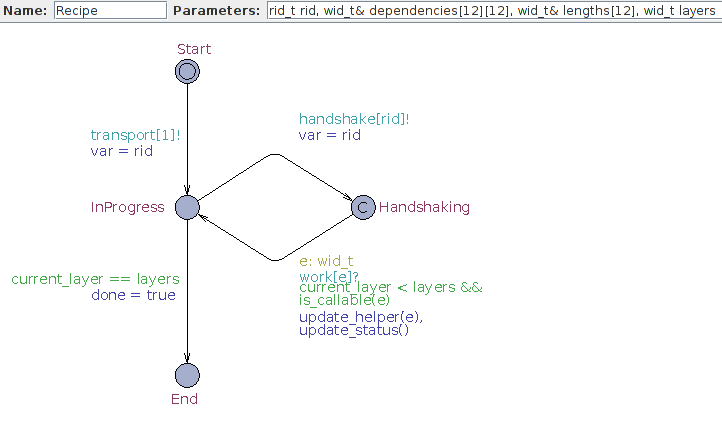
\includegraphics[width=0.8\textwidth]{images/firstrecipe.png}
\caption{Recipe Template}
\label{fig:firstrecipe}
\end{figure}

To represent an item passing through a FESTO factory, we design and implement the recipe template. This defines a set of steps that must be taken to create a specific product. A recipe synchronizes with a module to have work performed on it. Each module has a specific type of work, which it may perform on a recipe.  The recipe template can be seen in \cref{fig:firstrecipe}.

A recipe is initialized with an identifying id along with an array of arrays. This latter construct describes the dependency between steps that must be taken for a recipe to move to its end location. Each array layer describes a set of steps that may be taken in an arbitrary manner. However all these steps must be taken, before any of the steps in the next layer may be taken. For instance, the dependency structure [Hammer, Screw][Package], means that the given recipe should get hammered and screwed before it is packaged. However the hammering and screwing may occur in whatever sequence. 

When going from the start location a recipe will, through the transport channel, synchronize with the first module in the production line.  Through the global var variable the id of the recipe is passed to the module in order to lay claim on it. This is part of a simple mutual exclusion scheme, making sure that a module may only work on one specific recipe at a time. Once a recipe is in progress it may handshake with a module by using its id to identify itself. When identified, the module may perform a work action upon the recipe to complete a pending recipe step. If this is done, we make sure to mark the finished step as done, so that it is not repeated. In the case that all steps have been taken in a layer of the dependency array, we make sure to move onto the next. Once all layers have been completed,  we may pass to the end location. Here we set the local done variable to true. This is used to query our model checker to see,if we can reach a state where the recipe is finished. For a recipe named r1 the query would be: \[E<> r1.done\].

\subsection{Module}

\begin{figure}
\centering
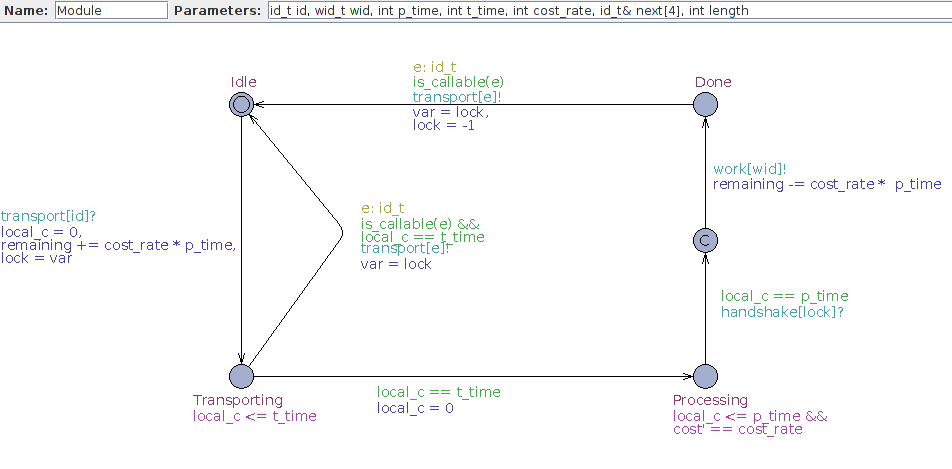
\includegraphics[width=0.8\textwidth]{images/firstmodule.png}
\caption{Module Template}
\label{fig:firstmodule}
\end{figure}

The module template models a module in a FESTO factory. A module is identified by its id parameter. A second parameter wid (work id) indicates the type of work the module may perform on a recipe. A module also includes  an array “next, which contains ids of modules, which it may pass an item onto. The module template can be seen in \cref{fig:firstmodule}.

To pass from the idle state, a module must receive an item from a module earlier in line by   synchronizing on the transport channel. As stated earlier, the first transport occurs between a recipe and the first module in line. This also passes the recipe id onto the module in order to lock other recipes out, saving the recipe id in the lock variable. From this point on, when a module synchronizes on transport, it passes the recipe id onto the next module for locking. After seizing to be idle the module waits for t\_time in the transport location. Afterwards it may synchronize on transport again to send the recipe to one of the next modules in line. Instead of passing on the recipe, we may try to work upon it. By giving the option of working or passing through, we simulate that some items don’t need to be worked on by every module in the production line. If we decide to work on the recipe, we go to the  processing location and wait for p\_time. Each time we delay by a single time unit in this location, the global cost variable is increased by the value of cost\_rate. Once time has passed, the module can identify its recipe through a handshake by using the recipe id saved in lock. Once it is confirmed that the module is working with the correct recipe, it will synchronize on the work channel, finishing its job upon the item. Once done the module may go back to the idle location by transporting the item to one of the next modules in line. 


\subsection{Remover}

\begin{figure}
\centering
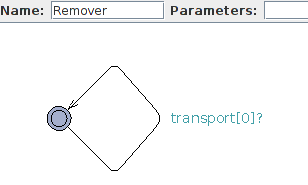
\includegraphics[width=0.8\textwidth]{images/firstremover.png}
\caption{Remover Template}
\label{fig:firstremover}
\end{figure}

The remover template is not very complex, and can be seen in \cref{fig:firstremover}. It continously tries to synchronize on the 0th transport channel to remove a recipe from the factory. The factory modules each have their own transport channel given by their id, which is 1 indexed. Thus a transport on 0 does not pass the recipe to a module, but instead to the remover. If we want to remove a recipe, when it is passed on from a specific module, we simply set one of the ids in the module’s next array to 0. Removing a recipe from a factory is especially beneficial in circular setups, as a finished recipe may otherwise keep being passed around. This may unnecessarily decrease factory throughput. By removing recipes. We also decrease the state space that needs to be searched by the model checker.  


\subsection{Coster}

\begin{figure}
\centering
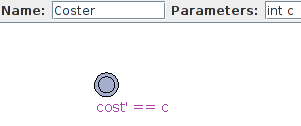
\includegraphics[width=0.8\textwidth]{images/firstcoster.png}
\caption{Coster Template}
\label{fig:firstcoster}
\end{figure}

The coster template ensures that parallel processing of recipes is prefered during a Best First Search. It can be seen in \cref{fig:firstcoster} The template is initialized with a rate c, which increases the global cost variable as a function of the global time passed. Without this, the search would have any reason to run several modules at the same time as the final cost would not change. By having a constant cost on the factory’s operating time, we make the prospect of parallel processing a prefered option.  



